

\begin{frame}[t]{Conclusão}
    \transboxout[duration=0.5]
    \framesubtitle{Mapa conceitual}    %\transboxin[duration=1,direction=30]

    \begin{figure}
        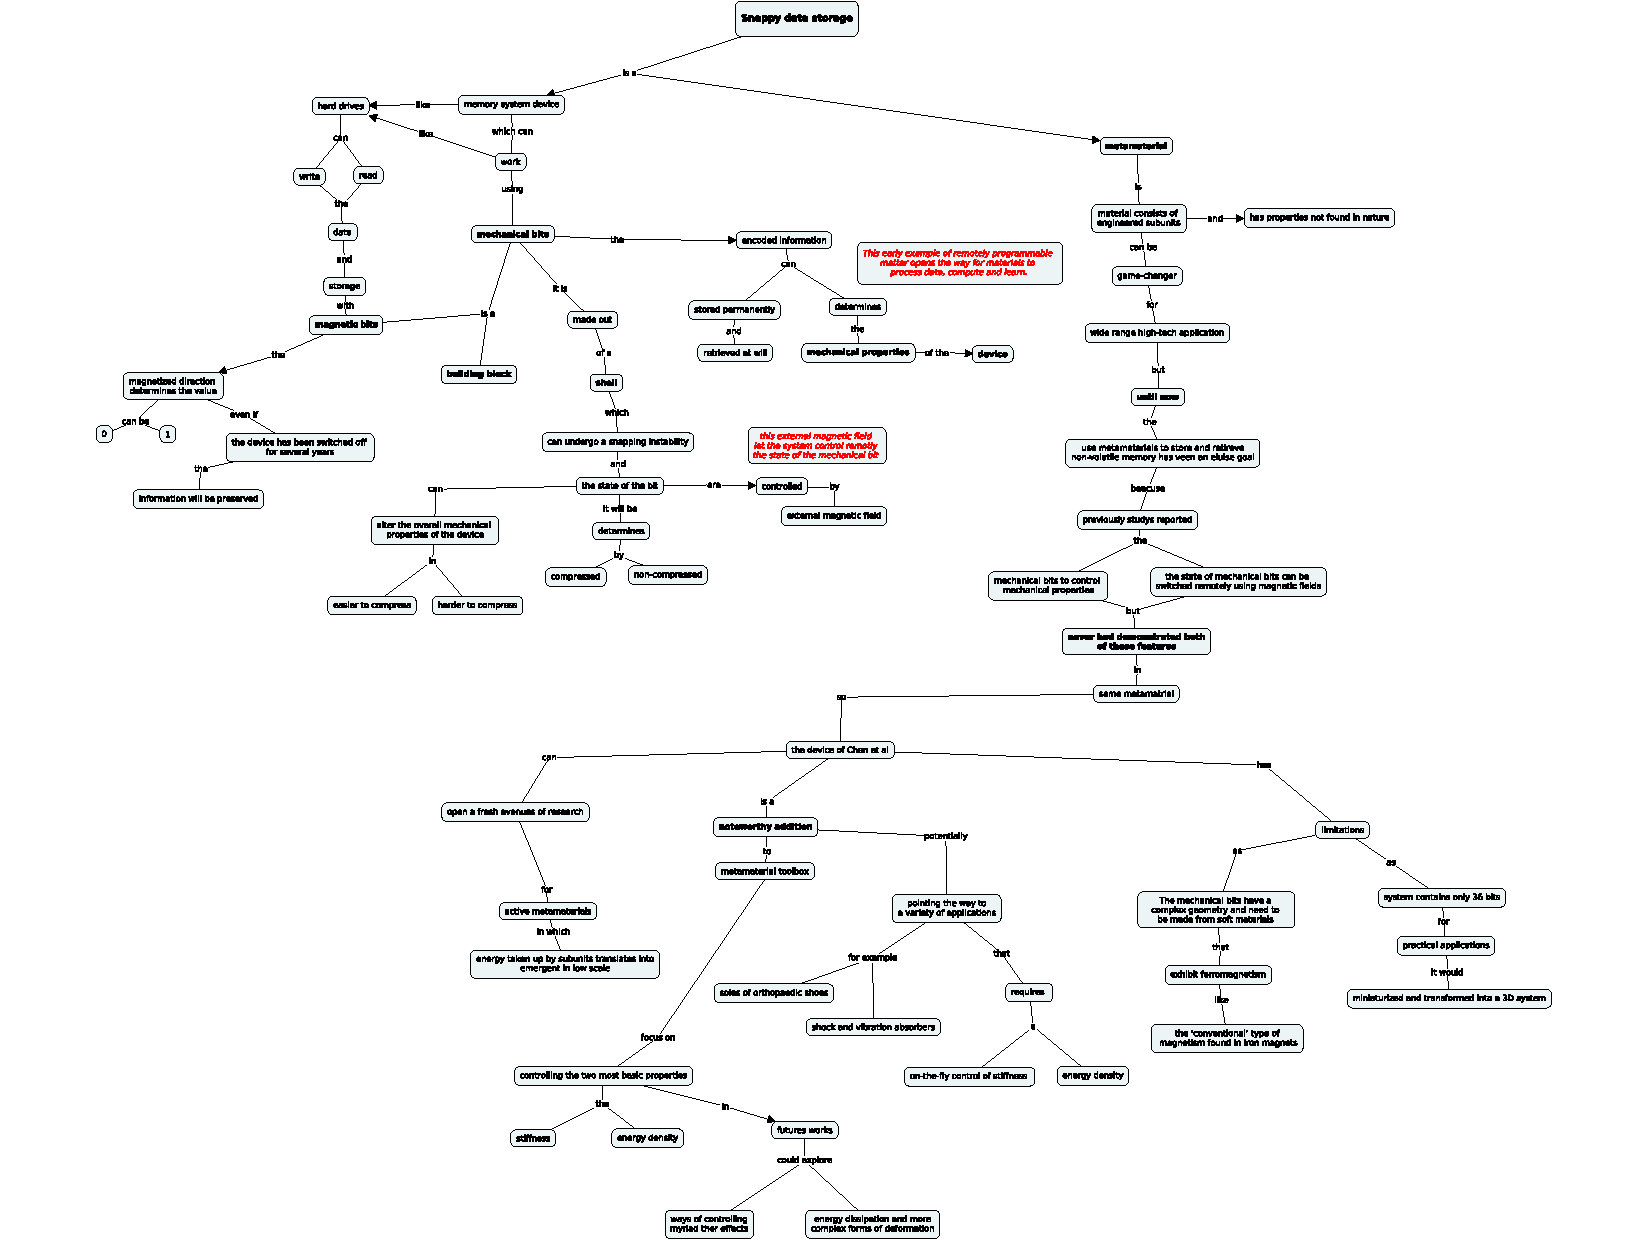
\includegraphics[width=0.55\textwidth]{concept-map.pdf}
        %\caption{.}
    \end{figure}
%*----------- notes
\end{frame}

\begin{frame}
    %\transdissolve[duration=0.5]
    %\hspace*{-1cm}

    \begin{columns}
        %\column{.01\textwidth}
        \column{0.4\textwidth}
        ~\hfill
        \vbox{}\vskip-1.4ex%
        \begin{beamercolorbox}[sep=8em, colsep*=18pt, wd=\textwidth,ht=\paperheight]{title page header}
            \begin{center}
                \huge{Fluxograma}
                \huge{de apresentação}
            \end{center}
        \end{beamercolorbox}%
        \column{.05\textwidth}
        \column{.6\textwidth}
        \begin{center}
            \begin{figure}
                \includegraphics[width=.7\textwidth]{chart.pdf}
            \end{figure}

        \end{center}

    \end{columns}

    %*----------- notes
\end{frame}

\begin{frame}[t]{Conclusão}
    \transboxout[duration=0.5]
    \framesubtitle{Roteiro de apresentação}    %\transboxin[duration=1,direction=30]

    \begin{figure}
        \includegraphics[width=.35\textwidth]{modelo-artigo.pdf}
        %\caption{.}
    \end{figure}
%*----------- notes
\end{frame}

%----------------------------------------------------SLIDE------------------
 \begin{frame}[t, allowframebreaks]{References}
 %\frametitle{References}
%\begin{frame}{Reference}
    %\transboxin[duration=1,direction=30]

    % \begin{bibunit}[plain]
    % %\cite{kanakia2012}
    % %\cite{agostini2007}
    % %\cite{azuma1997survey}
    % \cite{Buss2005}
  
    % \putbib
    % \end{bibunit}
  
    %\bibliographystyle{IEEEtran}
    %\bibliographystyle{IEEEtranS}
    %\bibliographystyle{IEEEbib}
    \bibliographystyle{abntex2-alf}
    %\bibliographystyle{abntex2-num}
    %\bibliographystyle{abnt-alf}
    \bibliography{bibliography} 
    %\putbib

%*----------- notes
    %\note[item]{Notes can help you to remember important information. Turn on the notes option.}
\end{frame}